\subsection{Material science}

A commonly used semiconductor for solar cells, is silicon. The supply of silicon is practically endless. 60\% of the Earth's crust is sand, for the major part SiO$_2$. Metallurgical grade silicon (MG-Si) is produced in large amounts to make special steel alloys. Its purity is only 99\% - insufficient for electronic applications \cite{solar_cells}. 

The semiconductor industry purifies this metallurgical-grade silicon until the purity is better than 99.99999~\%. This corresponds to less than 0.1~ppma (part per million atomic), meaning that the total number of foreign atoms must be less than 5$\cdot$10$^{15}$~cm$^{-3}$, due to silicon crystalline atoms density of 5$\cdot$10$^{22}$~cm$^{-3}$ \cite{solar_cells}.

Semiconductor-grade silicon is about ten times more pure than solar-grade silicon. That means that solar-grade silicon can contain up to 1~ppma impurities and still permit reasonably efficient cells. This allows for a lower cost purification process.

\subsubsection{Czochralski method}

The most common crystallization method used for both microelectronoic and photovoltaic industries is the Czochralski method (CZ) ,  shown in figure \ref{fig:czochralski_process} \cite{solar_cells}.

\begin{figure}[H]
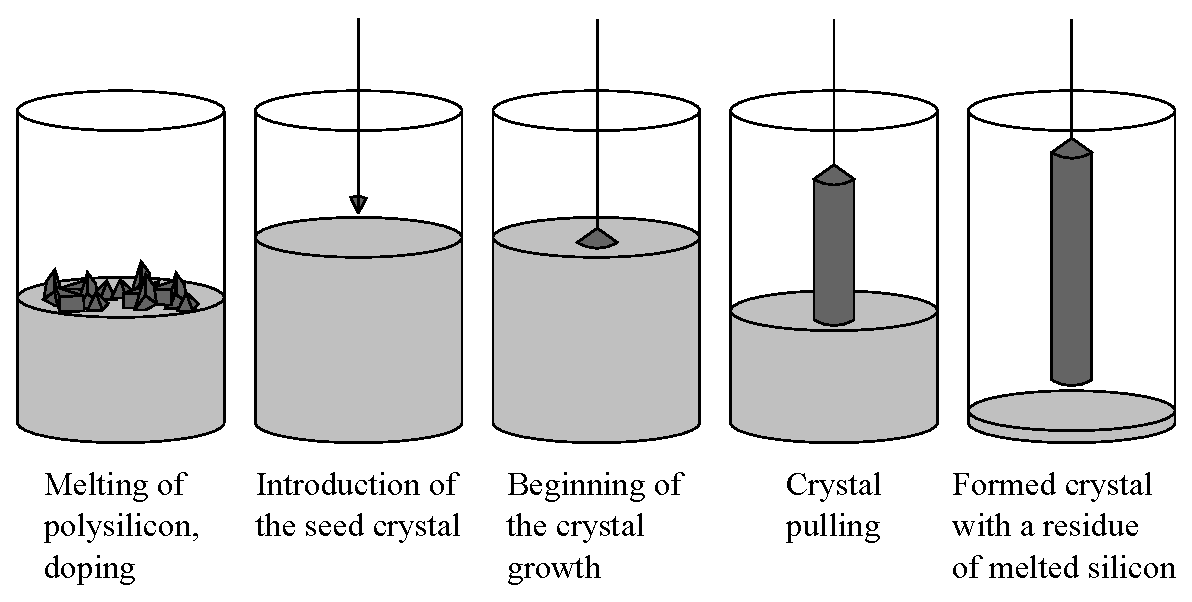
\includegraphics[width=\columnwidth]{Czochralski_Process}%
\caption{Czochralski process}%
\label{fig:czochralski_process}%
\end{figure}

In the CZ crystal growth, silicon chunks are first melted at 1414$^\circ$C in a graphite crucible lined with high purity quartz (SiO$_2$). This known as a feedstock. A small polysilicon crystal is used as a seed to start the crystallization process. The seed is carefully put in contact with the melt and then pulled out very slowly. The temperature is controlled, so that the silicon solidifies at the interface between the seed and the melt and the atoms arrange themselves according to the crystallographic structure of the seed. The crystal grows both vertically and laterally, aided by a rotation movement, yielding a cylindrical ingot of single-crystal silicon. 

The growth rate in the CZ method is about 5~cm/h and the cylindrical ingots are typically 1~m long, 20~cm in diameter and 75~kg in weight \cite{solar_cells}. A disadvantage of the CZ method is that the interaction between the molten silicon and the crucible introduces some contamintants, in particular carbon and oxygen. 

\subsubsection{Float-zone process}

The highest quality silicon crystals are obtained by using the float-zone process. In this method, the starting polysilicon is first given the shape of a cylindrical bar. The bar is then locally melted by a coil using radio frequency induction. By moving the coil, and hence the molten zone, along the bar starting from the seed end, the silicon adopts the crystalline structure. The molten zone is self-supporting and is never in contact with a foreign material, thus avoiding contamination problems. The typical growth rate is 15-30~cm/h, and the typical ingot is 15~cm in diameter and 1~m in length.

\subsubsection{Siemens process}

In the Siemens reactor process, trichlorosilane gas is introduced into a thermal decomposition furnace (reactor) exposing high-purity silicon rods at 1150~$^\circ$C. The trichlorosilane gas decomposes and deposits additional silicon onto the rods, enlarging them:

\begin{equation}
2 \text{HSiCl}_3 \rightarrow 2 \text{HCl} + \text{SiCl}_4
\label{eq:siemens}
\end{equation}

The silicon contained in the gas will deposit on the heated rods, which gradually grow until the desired diameter has been reached. The end product is in the form of rods or chunks of polysilicon. The technology in the Siemens reactor is widely implemented, accounting for a majority of the polysilicon production today, and produce a high purity material \cite{pv_handbook}.


\subsubsection{Multicrystalline silicon}

In order to reduce cost, and increase production rates, the multicrystalline silicon (mc-Si) production method was developed. It is possible to grow silicon ingots by simply melting the starting material, typically silicon scrap, into a crucible, and carefully controlling the cooling rate. Upon cooling, a directional solidification takes place and relatively large crystals grow in a columnar way. A crystalline seed is not used, and the nucleation of the silicon atoms commences in many places simultaneously, leading to a myriad of crystals (or grains) of arbitrary shape and crystallographic orientation. Each grain is several millimeters to centimeters across, and internally it has the same structure as single crystalline silicon. The boundaries between the different grains (grain boundaries), are the most obvious imperfection in the material, but they are not the only ones. Microdefect are also common and contamination from the crucible can happen as well, not to mention the possible impurities present in the starting silicon. This means that the mc-Si typically has lower electronic quality than the material produced by other methods, like the CZ method. Mc-Si typically contains much less oxygen then CZ-Si, due to CZ-Si is more exposed to air during the manufacturing process. The typical crystallization rate is 3.5~kg, and the growth cycle of a complete 16~kg ingot takes 46~h \cite{solar_cells}. 

\subsubsection{Wafers}

The silicon ingots have to be sliced into wafers. Before this they are shaped to meet dimensional specifications. The cylindrical CZ ingots are usually reduced to a quasi-square shape. This implies a loss of about 25~\% of the material, but is necessary if a high packing factor of the cells in the module is required. The large cast silicon parallelepipeds are sawn into smaller bricks. In the case of mc-Si ingots, the shaping is also used to discard the peripheral regions that are usually heavily contaminated by the crucible, which represents approximiately 15~\% of the ingot. In the photovoltaic industry, the wafers are cut by a multi-wire saw machines, that can cut simultaneously whole blocks, thus increasing the throughput dramatically (figure \ref{fig:wire_saw}).

\begin{figure}%
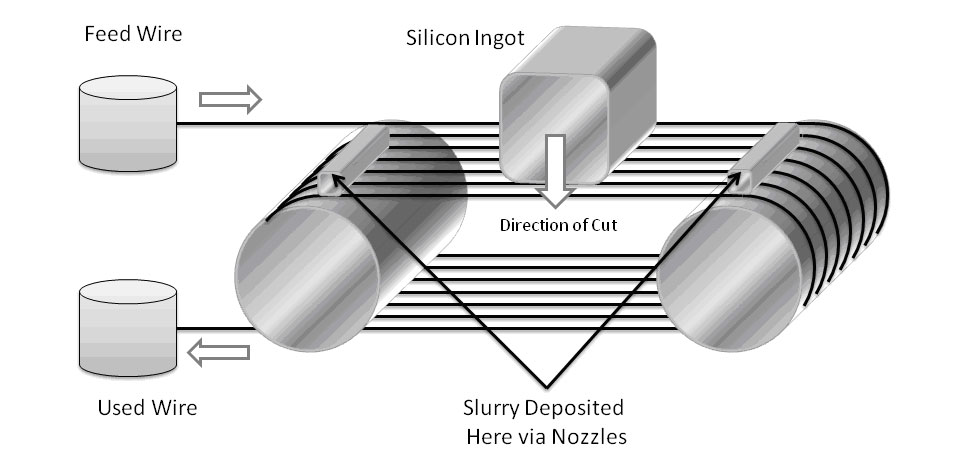
\includegraphics[width=\columnwidth]{wire_saw}%
\caption{Wafer wire saw (figure from \cite{wire_saw})}%
\label{fig:wire_saw}%
\end{figure}

An abrasive slurry helps the steel wires cut through silicon, which is a very hard material. The cutting is very slow, with eight hours being typically needed to cut through a 10x10~cm$^2$ block. Despite this advanced technique, slicing remains as one of the most costly steps of the whole silicon solar cell fabrication. Even if very thin wires are used, approximately 30~\% of the silicon is wasted as saw dust \cite{solar_cells}.


\subsubsection{Doping}

A controlled amount of boron or phosphorus is usually added to the melt (feedstock) to dope the silicon p- or n-type. Rather than the elemental boron or phosphorous, accurately measured amounts of silicon, heavily doped with those elements, are added to the melt. The typical boron concentration used for solar cell applications is 1.5$\cdot$10$^{16}$~cm$^{-3}$, which results in a resistivity of 1~\ohm cm \cite{solar_cells}.


\subsubsection{Defects}

Crystals possess imperfections. They are often referred to as crystalline defects. The presence of most of these crystalline defects is undesirable in silicon wafers. Crystalline defects may be classified into four categories according to their geometry; zero-dimensional or point defects, one-dimensional or line defects, two-dimensional or area defects, and three-dimensional or volume defects

\begin{table}[H]
\begin{tabular}{|c|c|}

\hline
\textbf{Defect type} & \textbf{Examples} \\ \hline

\multirow{4}{*}{Point or zero-dimensional defects} & Vacancy defects \\
 & Interstitial defects \\
 & Frenkel defects \\
 & Extrinsic defects \\ \hline
 
\multirow{2}{*}{Line or one-dimensional defects} & Straight dislocations (edge or screw) \\
 & Dislocation loops \\ \hline
 
\multirow{3}{*}{Area or two-dimensional defects} & Stacking faults \\
 & Twins \\
 & Grain boundaries \\ \hline

\multirow{2}{*}{Volume or three-dimentional defects} & Precipitates \\
 & Voids \\ \hline

\end{tabular}
\caption{Examples of crystalline defects from \cite{siliconfareast}}
\label{tab:crystalline_defects}
\end{table}

Vacancy defects are defects where a silicon atom is missing in the crystal structure. If an atom is located at a non-lattice location within the crystal, it is known as an interstitial defect. If the interstitial defect involves a silicon atom at an interstitial site within a silicon crystal, then it is referred to as a self-interstitial defect. Vacancies and self-interstitial defects are classified as intrinsic point defects \cite{siliconfareast}.
            
A Frenkel defect, is when an atom vacates its position in the crystal lattice to an interstitial position. Extrinsic point defects involve a foreign atom, and are more critical than intrinsic point defects. If this foreign atom replace a silicon atom in the lattice, it becomes a substitutional impurity. This include impurity atoms like the dopants B and P. Other common impurities are oxygen, carbon, and metals \cite{davies88}.


Dislocations, or crystal line defects consists of edge dislocations, screw dislocations or a combination of the two. Edge dislocation can be described as an extra plane of atoms squeezed into a part of the crystal lattice. The location with extra atoms would be under compressive stresses, while the part with correct number of atoms would be under tensile stresses. The line connecting all the atoms at the end of the extra plane is known as the dislocation line.

Screw dislocation is such that a step or ramp is formed by the displacement of atoms in a plane in the crystal. The dislocation line of a screw dislocation is in the axis of the screw.


\begin{figure}[H]
\centering
\subfigure[An edge dislocation]{
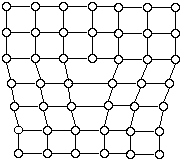
\includegraphics[width=.45\columnwidth]{edge_dislocation}
\label{fig:edge_dislocation}
}
\subfigure[A screw dislocation from \cite{siliconfareast}]{
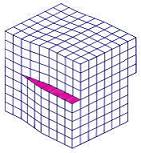
\includegraphics[width=.45\columnwidth]{screw_dislocation}
\label{fig:screw_dislocation}
}
\label{fig:dislocations}
\caption{Dislocations}
\end{figure}

Dislocation loop is a closed curve consisting of an extra plane of atoms lying entirely within the crystal. The line usually form a circular shape, since this shape results in the lowest dislocation energy \cite{siliconfareast}.

Dislocations are not wanted in silicon wafers because impurities are known as recombination centers \cite{tarasov00} and serve as sinks for metallic impurities. Gettering may also occur at dislocations, which can lead to the formation of precipitates.


Stacking faults can be considered as a disturbance in the regularity of the stacking of planes in a crystal lattice. This can occur when a plane is inserted or removed from the lattice. Stacking faults can become electrically active when decorated by impurity atoms. Such stacking faults can lead to device degradation.

A twin is a mirroring of a regular lattice formed during the growth of the silicon ingot. This is usually caused by perturbation. The twin boundary is the mirror plane of the twin formation as seen in figure (\ref{fig:twin_boundary});

\begin{figure}[H]
\centering
\subfigure[Stacking faults from \cite{stacking_faults}]{
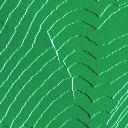
\includegraphics[width=.45\columnwidth]{stacking_fault}
\label{fig:stacking_faults}
}
\subfigure[Twin boundary]{
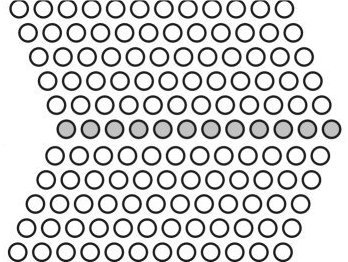
\includegraphics[width=.45\columnwidth]{twin_boundary}
\label{fig:twin_boundary}
}
\label{fig:dislocations_types}
\caption{Area defects}
\end{figure}

Grain boundaries are the boundary in between individual grains where crystal orientation is different from one another. This is common in mc-Si samples due to the production method.
     
Bulk or volume defects include voids and precipitates of extrinsic and intrinsic point defects. Impurities in a crystal which are introduced at a high temperature usually have a higher solubility than for lower temperatures. If the maximum concentration of an impurity allowed by its solubility at high temperature, the crystal become supersaturated with that impurity once it is cooled down. Under such supersaturated conditions, the crystal seeks and achieves equilibrium by precipitating the excess impurity atoms into another plane phase of different composition or structure. Precipitates are undesireable because they can act as sites for generation of dislocations. Precipitates can form in silicon from metallic impurities, oxygen and dopants like boron \cite{siliconfareast}.

